\documentclass[a4paper,12pt]{report}
\usepackage
[
a4paper,
left=4cm,
right=2.5cm,
top=3cm,
bottom=4cm,
]
{geometry}
\usepackage[czech]{babel}
\usepackage[utf8]{inputenc}
\usepackage[T1]{fontenc}
%\usepackage{hyperref}
\usepackage{xcolor} % barevný text - vyšedění
\usepackage{amsmath}
\usepackage{amssymb}
\usepackage{amsthm}
%\usepackage[toc,page]{appendix}
\usepackage{mdframed}
\usepackage{graphicx}
%\usepackage{subfigure}  % abych mohl dát 2 obrázky vedle sebe
\usepackage[font=footnotesize,labelfont=bf,justification=centering]{caption} % 2 obrázky vedle sebe, nastavuje font a centruje caption nad tabulkama a u obrázků
\usepackage[font=scriptsize]{subcaption}
\captionsetup{font=footnotesize}

%\usepackage{titlesec}
\usepackage{icomma} %nedělá za čárkou v číslech automaticky mezeru
\usepackage{url}
\usepackage{float}
\usepackage{enumerate} % hezky číslované listy (např. římská čísla)
%\usepackage[justification=centering]{caption} 

\usepackage{listings}
\usepackage{booktabs}

\newtheorem{theorem}{Věta}[chapter]
\newtheorem*{theoremnon}{Věta}
\newtheorem{lemma}{Lemma}[chapter]
\newtheorem{corollary}{Důsledek}[chapter]
%\theoremstyle{definition}
\newtheorem{definition}{Definice}[chapter]
\newtheorem*{defnon}{Definice}
\newtheorem{problem}{Úloha}[chapter]
\theoremstyle{remark}
\newtheorem{remark}{Poznámka}[chapter]

\renewcommand\qedsymbol{$\blacksquare$} % plný čtvereček za důkazem



\setlength{\topmargin}{-.25in}
\setlength{\parindent}{0pt}
\setlength{\parskip}{0.5\baselineskip}

%\usepackage{titlesec}
%\titleformat{\chapter}
%{\normalfont\LARGE}{\thechapter}{1em}{}
%\titlespacing*{\chapter}{0pt}{3.5ex plus 1ex minus .2ex}{2.3ex plus .2ex}

% Obecná definice pro styl nadpisů kapitol, sekcí atd. 
\usepackage{titlesec, blindtext, color}
\definecolor{gray75}{gray}{0.75}
\newcommand{\hsp}{\hspace{20pt}}

% Definice stylu pro chapter title
\titleformat{\chapter}[hang]{\Huge\bfseries}{\thechapter\hsp\textcolor{gray75}{|}\hsp}{0pt}{\Huge\bfseries}
% Definice stylu pro chapter title - bez číslování
\titleformat{name=\chapter,numberless}[hang]{\Huge\bfseries}{\hsp\textcolor{gray75}{|}\hsp}{0pt}{\Huge\bfseries}
% Definice stylu pro section title
\titleformat{\section}[hang]{\Large\bfseries}{\thesection\hsp\textcolor{gray75}{|}\hsp}{0pt}{\Large\bfseries}

\definecolor{identifiercolor}{rgb}{.4,.6,.56}
\definecolor{stringcolor}{gray}{0.5}
\definecolor{inactivecolor}{rgb}{0.15,0.15,0.5}
\usepackage{listings}
\lstset{basicstyle={\footnotesize\def\fvm@Scale{.85}\fontfamily{fvm}\selectfont},
	breaklines=true,
	escapeinside={\%*}{*)},
	keywordstyle={\bfseries\color{inactivecolor}},
	stringstyle={\bfseries\color{stringcolor}},
	identifierstyle={\bfseries\color{identifiercolor}},
	language=Mathematica,
	otherkeywords={DiscretizeRegion},
	showstringspaces=false}
\renewcommand{\lstlistingname}{Listing}


%%%%%%%% per partes
\ExplSyntaxOn
\NewDocumentCommand{\byparts}{O{0pt}m}
{
	\keys_set:nn { elisabeth/byparts } { #2 }
	\elisabeth_byparts:n { #1 }
}

\keys_define:nn { elisabeth/byparts }
{
	x  .tl_set:N = \l__elisabeth_byparts_u_tl,
	x' .tl_set:N = \l__elisabeth_byparts_up_tl,
	y  .tl_set:N = \l__elisabeth_byparts_v_tl,
	y' .tl_set:N = \l__elisabeth_byparts_vp_tl,
}

\cs_new_protected:Nn \elisabeth_byparts:n
{
	\begin{vmatrix}\,\begin{aligned}
			x\hphantom{'} &= \l__elisabeth_byparts_u_tl
			&
			y' &= \l__elisabeth_byparts_vp_tl
			\\[#1]
			x' &= \l__elisabeth_byparts_up_tl
			&
			y\hphantom{'} &= \l__elisabeth_byparts_v_tl
		\end{aligned}\,\end{vmatrix}
}

\ExplSyntaxOff
%%%%%%%%%%%%%%%%%


\title{
	{
\includegraphics[width=\linewidth]{FAV_logo.jpg}}\\[2cm]
	{Lineární řešiče v OpenFOAM}\\	
	{\small{Semestrální práce}}\\
	{\small{KMA/PVM}}\\
}

\author{Jan Půlpán}


\begin{document}
	\maketitle

	{\let\clearpage\relax \chapter{Teoretický úvod}}



	
	OpenFOAM je sada výpočetních nástrojů pro numerické simulace CFD (computational fluid dynamics) problémů, tedy problémů zabývajících se prouděním tekutin, vedením tepla a podobných procesů. OpenFOAM využívá k hledání řešení metody konečných objemů (FVM). 
	
	FVM je numerická metoda na řešení parciálních diferenciálních rovnic na dané 3D geometrii převedené na síť nepřekrývajích se elementů (konečných objemů). Tu pak pomocí diskretizace převedeme na soustavu algebraických rovnich, kterou řešíme pomocí lineárních řešiců a výsledné řešení obsahuje hodnotu sledovaných proměnných pro každý z těchto elementů.
	
	Budeme se zabývat jen posledním článkem řetězce, tedy lineárními řešiči. Na testovací úloze si ukážeme vhodnost jednotlivých řešičů a budeme sledovat vliv parametrů na konvergenci řešení. Úkolem lineárních řešičů (dále budeme používat jen \uv{řešičů}, pokud nebude hrozit záměna kontextu) je najít řešení soustavy algebraických rovnic tvaru
	\begin{equation}
		\boldsymbol{A}\boldsymbol{x} = \boldsymbol{b},
		\label{eq:linear_set}
	\end{equation}
	kde $\boldsymbol{A}$ je regulární matice popisující diskretizovaný model, $x$ vektor závislé proměnné a $b$ vektor pravé strany. 
	
	Pokud matice $\boldsymbol{A}$ umožňuje snadnou inverzi, je nejjednodušší získat přesné řešení soustavy přímým řešičem vztahem 
	$$ \boldsymbol{x} = \boldsymbol{A}^{-1} \boldsymbol{b}.$$ 
	Většinou ale nejde inverzi snadno nalézt a v tom případě se používají přibližné řešiče iterační. První možností jsou stacionární iterační metody, kdy matici $\boldsymbol{A}$ můžeme rozdělit (například pomocí $LU$ rozkladu) na $\boldsymbol{A} = \boldsymbol{M} - \boldsymbol{N}$. matice $\pmb{M}$ musí být snadno invertovatelná a řešení pak hledáme poomocí iterací 
	
	\begin{equation}
		\boldsymbol{x^{(k+1)}} = \boldsymbol{M}^{-1}(\boldsymbol{N}\boldsymbol{x^{(k)}} + \boldsymbol{b})
		\label{eq:stat_iter}
	\end{equation}

	Pevný bod operátoru \eqref{eq:stat_iter} je pak přesným řešením soustavy \eqref{eq:linear_set}.  
	
	Druhou používanou metodou iteračních řešičů jsou metody Krylovových podprostorů. Hledáme tak přibližné řešení v podprostorech s rostoucí dimenzí generovaných čtvercovou maticí $\boldsymbol{A}$ a vektorem $\boldsymbol{b}$. Krylovův podprostor $r$tého řádu je definován jako 
	$$\mathcal{K}_r(\boldsymbol{A},\boldsymbol{b}) = \textrm{span}\{\boldsymbol{b}, \boldsymbol{Ab}, \boldsymbol{A}^2\boldsymbol{b}, \dots, \boldsymbol{A}^{r-1}\boldsymbol{b}\}.$$
	TROCHU LÍP POPSAT, KOUKNOUT DO NA
	
	Iterační metody obecně měří chybu aproximace řešení pomocí reziduí, tedy dosazením aproximovaného řešení do původních rovnic a vypočtením rozdílu oproti pravé straně $\boldsymbol{b}$. Reziduum $\boldsymbol{r}$ definujeme jako 
	\begin{equation}
		\boldsymbol{r} = \boldsymbol{b}-\boldsymbol{A}x.
		\label{eq:residuum}
	\end{equation} 
	
	
	Často se při numerickém řešení lineárních algebrických rovnic používá \textbf{předpodmínění}, které zajistí rychlejší šíření informace na síti. Při levém předpodmínění (existuje i pravé a centrální) předpokládáme soustavu ve tvaru
	$$\boldsymbol{M}^{-1}\boldsymbol{A}\boldsymbol{x} =\boldsymbol{M}^{-1}\boldsymbol{b}$$
	kde $\boldsymbol{M}$ je předpodmiňovač. Ten zajistí, že konvergence předpodmíněného systému je rychlejší, než bez něj. $\boldsymbol{M}$ je často uvažována jako snadno invertovatelná aproximace matice $\boldsymbol{A}$. Nejjednodušší volbou je tak $\boldsymbol{M} = \boldsymbol{I}$, což ovšem vede k nepodmíněnému problému. Ideální je naopak $\boldsymbol{M} = \boldsymbol{A}$, to ovšem znamená, že inverze předpodmiňovače je stejně náročná jako původní matice.
	

	Ke zlepšení konvergence se u lineárních řešičů využívá často i tzv. \textbf{smoother}. Jacobiho, nebo Gauss-Seidelova metoda jsou často využívány jako smoother. Po každé iteraci řešiče metody se pustí několik iterací vybraného smootheru, který \uv{vyhladí} špičku v reziduu a tím i sníží jeho normovanou hodnotu. Na rozdíl od předpodmínění dokáže smoother snížit závislost sítě na počtu iterací. Gaussův-Seidelův smoother používá například následujícího vztahu
	
	\begin{equation}
		\boldsymbol{x^{(k+1)}} = \boldsymbol{x^{(k)}}+\boldsymbol{L}^{-1}(\boldsymbol{b} -  \boldsymbol{A}\boldsymbol{x^{(k)}}),
		\label{eq:gs_smoother}
	\end{equation}

kde $\boldsymbol{L}$ je dolní trojúhelníková část matice $\boldsymbol{A}$.
	
	
	{\let\clearpage\relax \chapter{Lineární řešiče v OpenFOAM}}

OpenFOAM obsahuje kromě základního přímého řešiče \texttt{diagonalSolver} tři základní typy řešičů:
\begin{enumerate}
	\item řešiče metodou konjugovaných gradientů 
	\item smooth řešiče
	\item multigrid řešiče
\end{enumerate}

Jednotlivé řešiče jsou popsány v tabulce \ref{table:solvers}.

\begin{table}[H]
	\centering
	\caption{řešiče v rámci OpenFOAM}
	\renewcommand{\arraystretch}{1.7}
	\begin{tabular}{*3l}
		\toprule
		\textbf{Řešič} & \textbf{Označení}&\textbf{Matice $\boldsymbol{A}$}\\
		\midrule
		{\small Preconditioned conjugate gradient}& PCG& sym\\
		{\small Preconditioned bi-conjugate gradient}& PBiCG&asym \\		
		{\small Stabilized Preconditioned (bi-)conjugate gradient}& PBiCGStab&sym/asym  \\
		{\small Solver using a smoother}& smoothSolver&sym/asym \\
		{\small Generalised geometric-algebraic multi-grid}& GAMG&sym/asym  \\
		{\small Diagonal solver for explicit systems}& 	diagonal \\
	
		\bottomrule
	\end{tabular}
	
	\label{table:solvers}
\end{table}
		
To který řešič je možné použít je závislé na matici $\boldsymbol{A}$ a tom, jestli je symetrická nebo nesymetrická. Symetrie $\boldsymbol{A}$ samozřejmě závisí na rovnicích, které chceme řešit. V případě, že zvolíme nesprávný řešič vzhledem k symetričnosti matice $\boldsymbol{A}$ OpenFOAM sám volbu opraví.

Reziduum je během jednotlivých iterací vyhodnocováno pomocí vztahu \eqref{eq:residuum}. Každý řešič má k reziduu trochu jíný přístup, obecně ale dochází k normalizaci a škálování rezidua vztahy

$$n = \sum \left( | \boldsymbol{A}x - \boldsymbol{A}\hat{x} | + | \boldsymbol{b} - \boldsymbol{A}\hat{x} | \right),$$
$$r = \frac{1}{n} \sum | \boldsymbol{b} - \boldsymbol{A}x |.$$ 

Pro každý typ řešice se nastaví parametr pro velikost rezidua (\texttt{tolerance}) a také relativní toleranci (\texttt{relTol}) pro poměr aktuálního rezidua v rámci jedné iterace a počátečního rezidua před začátkem iterace. Řešič se následně zastaví pokud je splněna alespoň jedna z těchto podmínek:
\begin{enumerate}
	\item reziduum je menší než nastavená \texttt{tolerance},
	\item relativní tolerance je menší než nastavená \texttt{relTol},
	\item je dosaženo nastaveného maximálního počtu iterací \texttt{maxIter}.
\end{enumerate}


Metoda sdružených gradientů (conjugent gradients) - PCG. PBiCG, PBiCGStab

Metoda sdružených gradientů (CG) je iterační algoritmus řešení soustav lineárních rovnic, který využívá sdružených směrů a vyžaduje symetrickou matici (postivně definitní) matici $\boldsymbol{A}$. Proto vznikla i metoda "bi-conjugate gradients" (dvojitých sdružených směrů), která pracuje s asymetrickými maticemi. OpenFoam obsahuje řešiče PCG a PBiCG s implementací těchto řešičů. Obě varianty jsou předpodmíňěné. Navíc je obsažen i PBiCGStab řešič, který umí pracovat se symetricvkou i nesymetrickou maticí $\boldsymbol{A}$.

Předpodmičovač je volitelný a obsahuje následující možnosti:

Preconditioner	Keyword
Diagonal incomplete-Cholesky (symmetric)	DIC
Faster diagonal incomplete-Cholesky (DIC with caching)	FDIC
Diagonal incomplete-LU (asymmetric)	DILU
Diagonal	diagonal
Geometric-algebraic multi-grid	GAMG
No preconditioning	none



NĚCO O SMOOTH ŘEŠIČÍCH 

The solvers that use a smoother require the smoother to be specified. The smoother options are listed in Table 6.11. Generally GaussSeidel is the most reliable option, but for bad matrices DIC can offer better convergence. In some cases, additional post-smoothing using GaussSeidel is further beneficial, i.e. the method denoted as DICGaussSeidel


Smoother	Keyword
Gauss-Seidel	GaussSeidel
Diagonal incomplete-Cholesky (symmetric)	DIC
Diagonal incomplete-Cholesky with Gauss-Seidel (symmetric)	DICGaussSeidel





NĚCO O MULTIGRID ŘEŠIČÍCH (MULTIGRID METODY)

The generalised method of geometric-algebraic multi-grid (GAMG) uses the principle of: generating a quick solution on a mesh with a small number of cells; mapping this solution onto a finer mesh; using it as an initial guess to obtain an accurate solution on the fine mesh. GAMG is faster than standard methods when the increase in speed by solving first on coarser meshes outweighs the additional costs of mesh refinement and mapping of field data. In practice, GAMG starts with the mesh specified by the user and coarsens/refines the mesh in stages. The user is only required to specify an approximate mesh size at the most coarse level in terms of the number of cells nCoarsestCells.


NĚCO O RESIDUAL CONTROL

By default, cases will run until the time settings are achieved in the case controlDict dictionary. Alternatively, the residualControl object can be added to the fvSolution dictionary to enable additional controls. This operates in two modes:

Steady state
To terminate the case when the initial residual of the field equations falls below user-specified threshold values for SIMPLE-based solvers:

residualControl
{
	p           1e-2;
	"(Ux Uy)"   1e-4;
	"(k|epsilon|omega)" 1e-4;
}


NĚCO O RELAXACI

under-relaxation, a technique used for improving stability of a computation, particularly in solving steady-state problems. Under-relaxation works by limiting the amount which a variable changes from one iteration to the next, either by modifying the solution matrix and source prior to solving for a field or by modifying the field directly. An under-relaxation factor $\alpha, 0 < \alpha \leq 1$  specifies the amount of under-relaxation, ranging from none at all for $\alpha = 1$  and increasing in strength as $\alpha -> 0$ The limiting case where $\alpha =  0$  represents a solution which does not change at all with successive iterations. An optimum choice of $\alpha$  is one that is small enough to ensure stable computation but large enough to move the iterative process forward quickly; values of $\alpha$   as high as 0.9 can ensure stability in some cases and anything much below, say, 0.2 are prohibitively restrictive in slowing the iterative process


\begin{enumerate}
	\item jaké jsou možnosti, jaké jsou parametry
	\begin{enumerate}
		\item     diagonalSolver - pokud je matic A diagonální, pak vypočítám $A^{-1} = A/diag(A)$ a jsem hotov (https://www.openfoam.com/documentation/guides/latest/doc/guide-solvers.html)
	\end{enumerate}
\end{enumerate}





	{\let\clearpage\relax \chapter{Porovnání řešičů}}
	
	Lineární řešiče porovnáme na konkrétní úloze stacionárního proudění v lopatkové mříži. Zachováme přitom jednotné parametry nastavení úlohy až na nastavení jednotlivých lineárních řešičů. Zajímat nás bude konvergence řešení a výpočetní náročnost. Zadání úlohy je na obrázku \ref{fig:zadani}, který definuje geometrii úlohy i okrajové podmínky. 
	
	\begin{figure}[H]
		\centering
		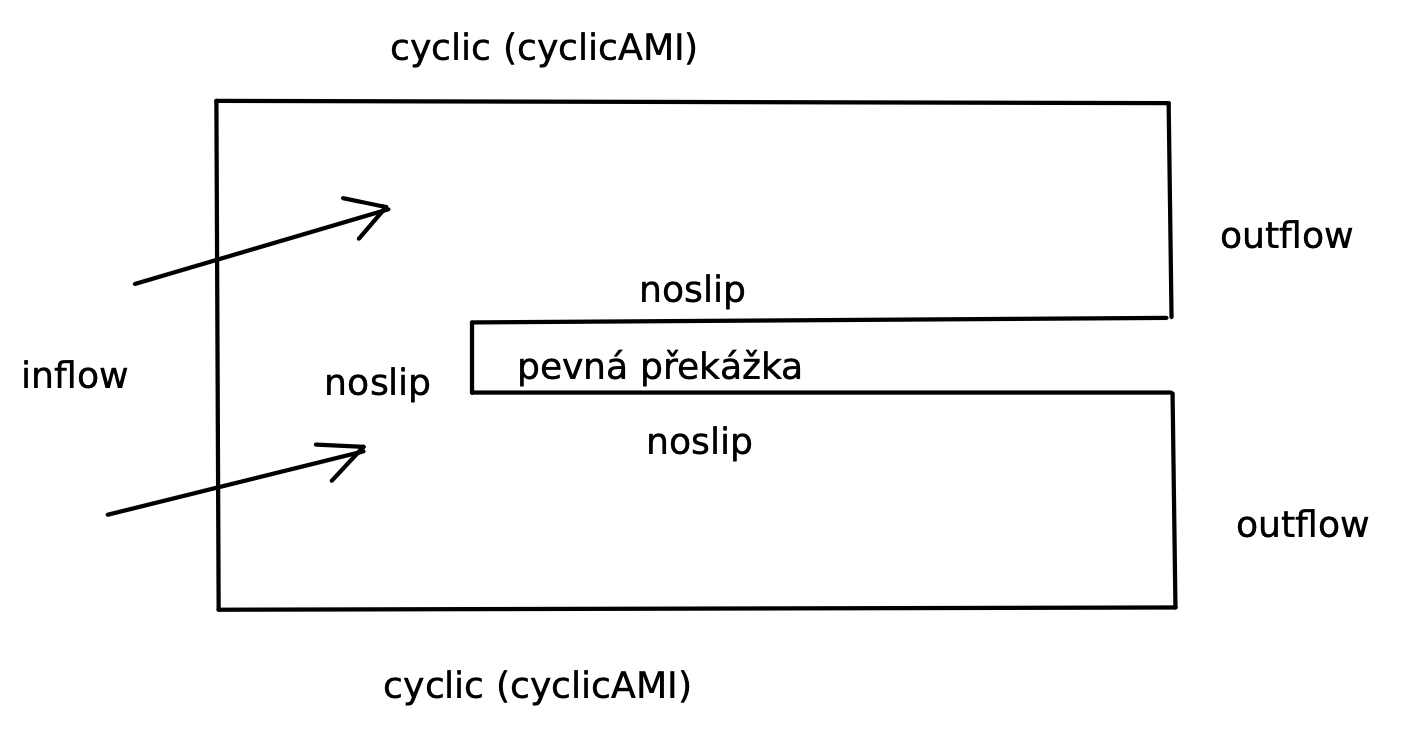
\includegraphics[width=1\linewidth]{zadani.png}
		\caption{Popis řešeného modelu}
		\label{fig:zadani}
	\end{figure}


Nejprve musíme definovat síť na které budeme naši úlohu řešit. Úloha je v 2D, ale OpenFOAM řeší vše ve 3D. Třetí souřadnici tedy nastavíme minimální, jen jako jednu buňku, a budeme ji ve výsledcích vlastně ignorovat.  Nejvíce se toho bude dít kolem \uv{vykousknuté} části a proto v těchto místech síť uděláme hustší jak je vidět na obrázku \ref{fig:pvmesh-detail}. Celá síť je pak na obrázku \ref{fig:pvmesh} a obsahuje celkem $108800$ jednotlivých buněk, na kterých budeme úlohu numericky integrovat. Konkrétní definice je v souboru \texttt{blockMeshDict} v příloze \ref{app:blockmeshdict}.

\begin{figure}[H]
	\centering
	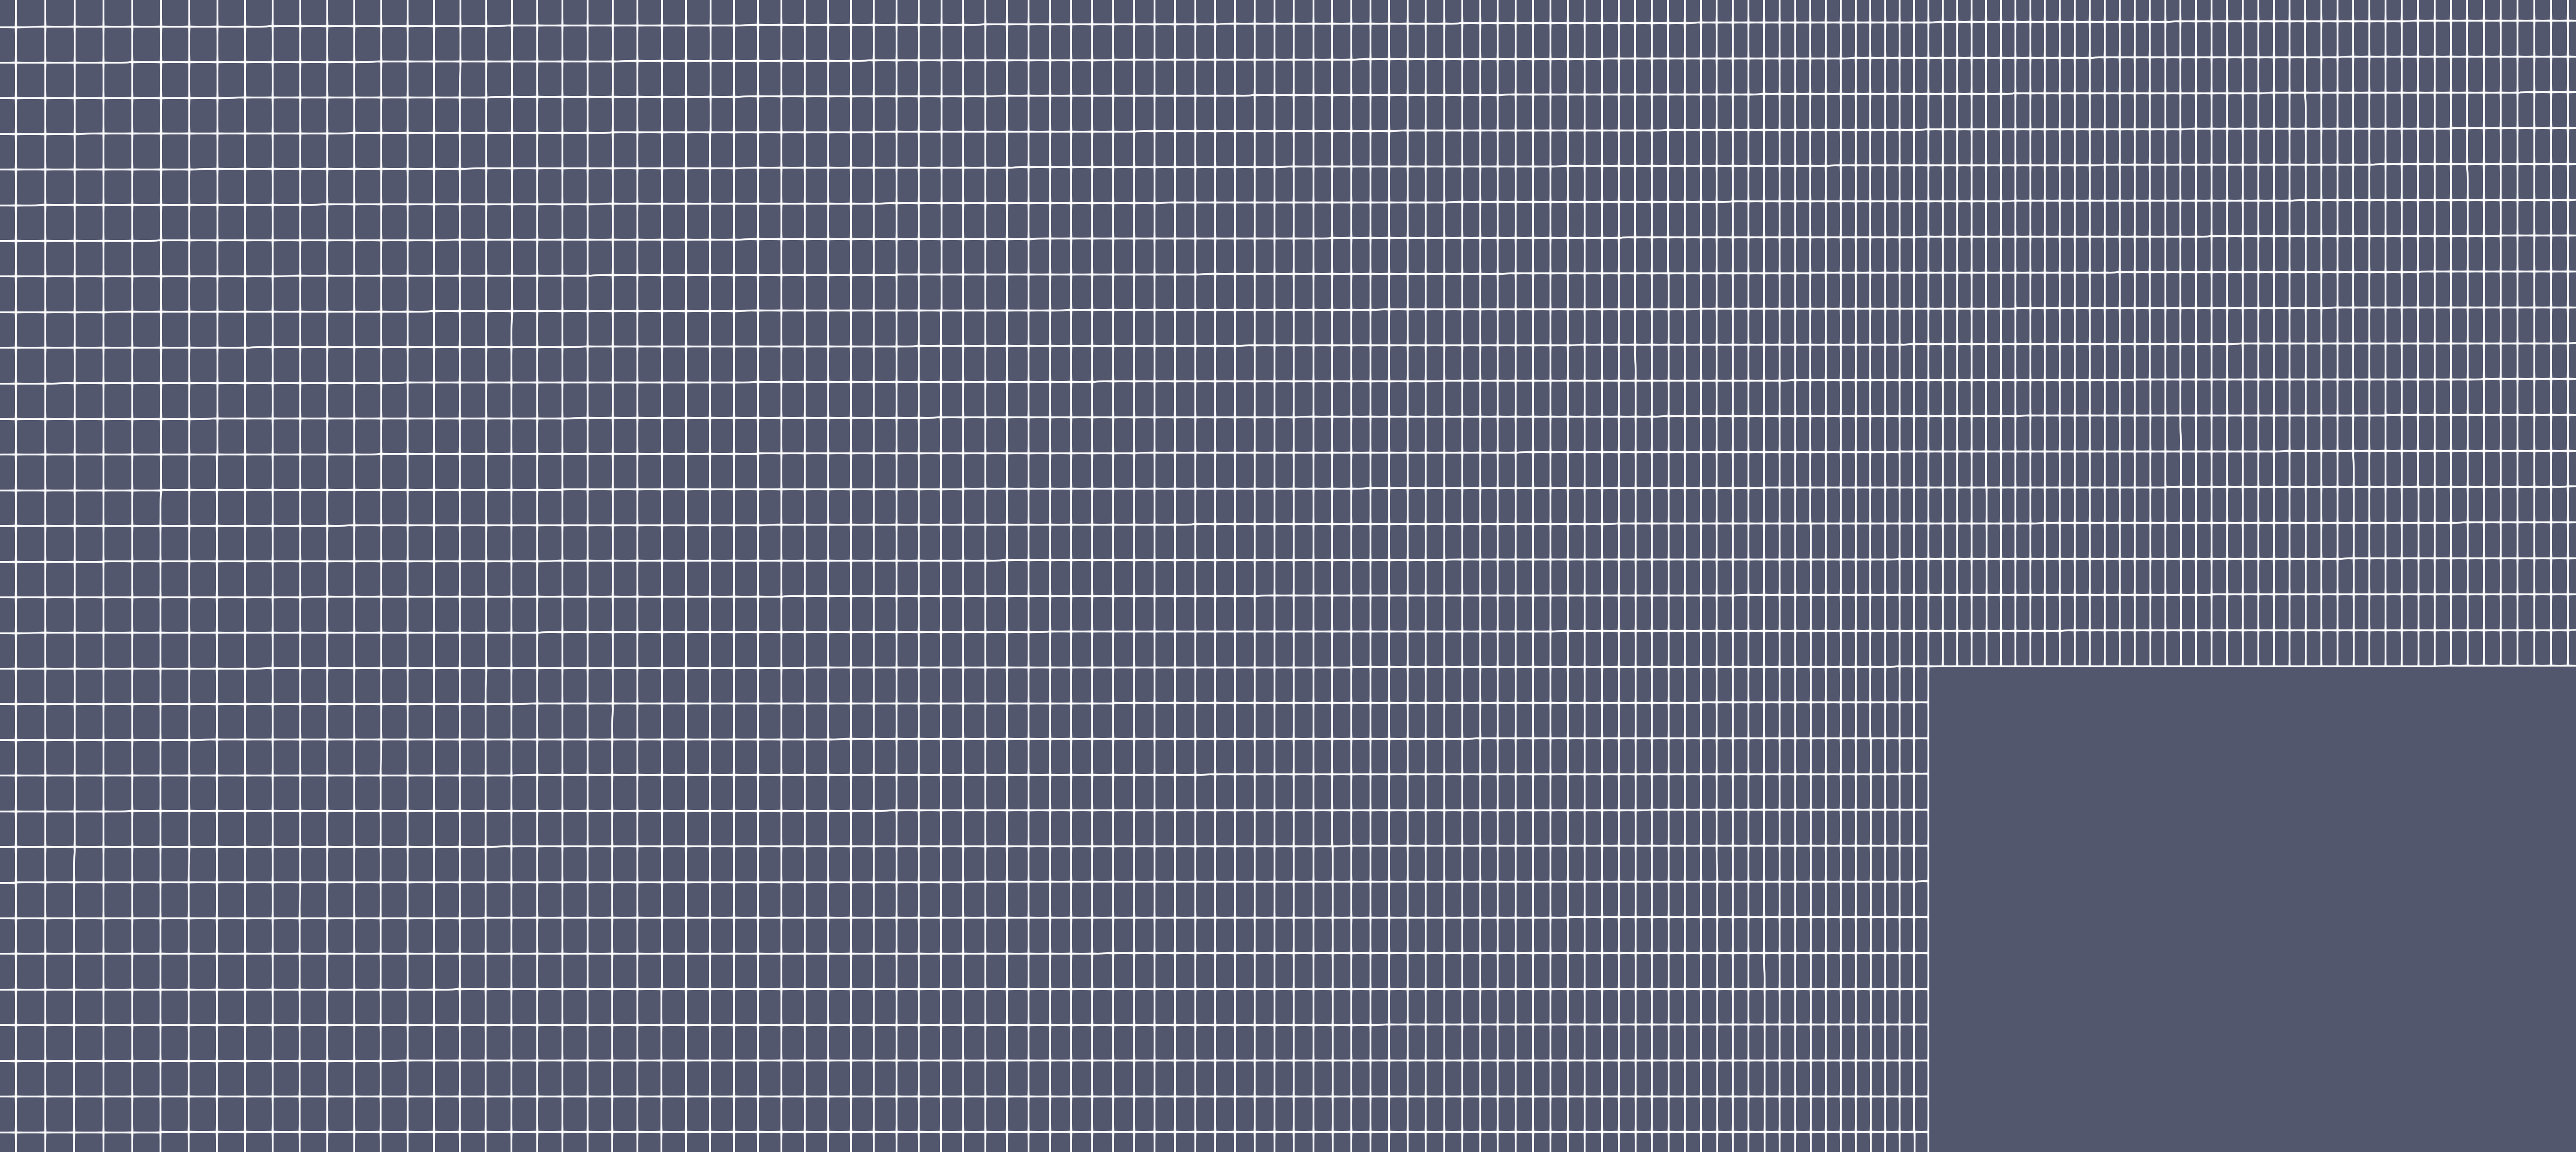
\includegraphics[width=1\linewidth]{pv-mesh-detail.png}
	\caption{Detail sítě řešeného modelu}
	\label{fig:pvmesh-detail}
\end{figure}



\begin{figure}[H]
	\centering
	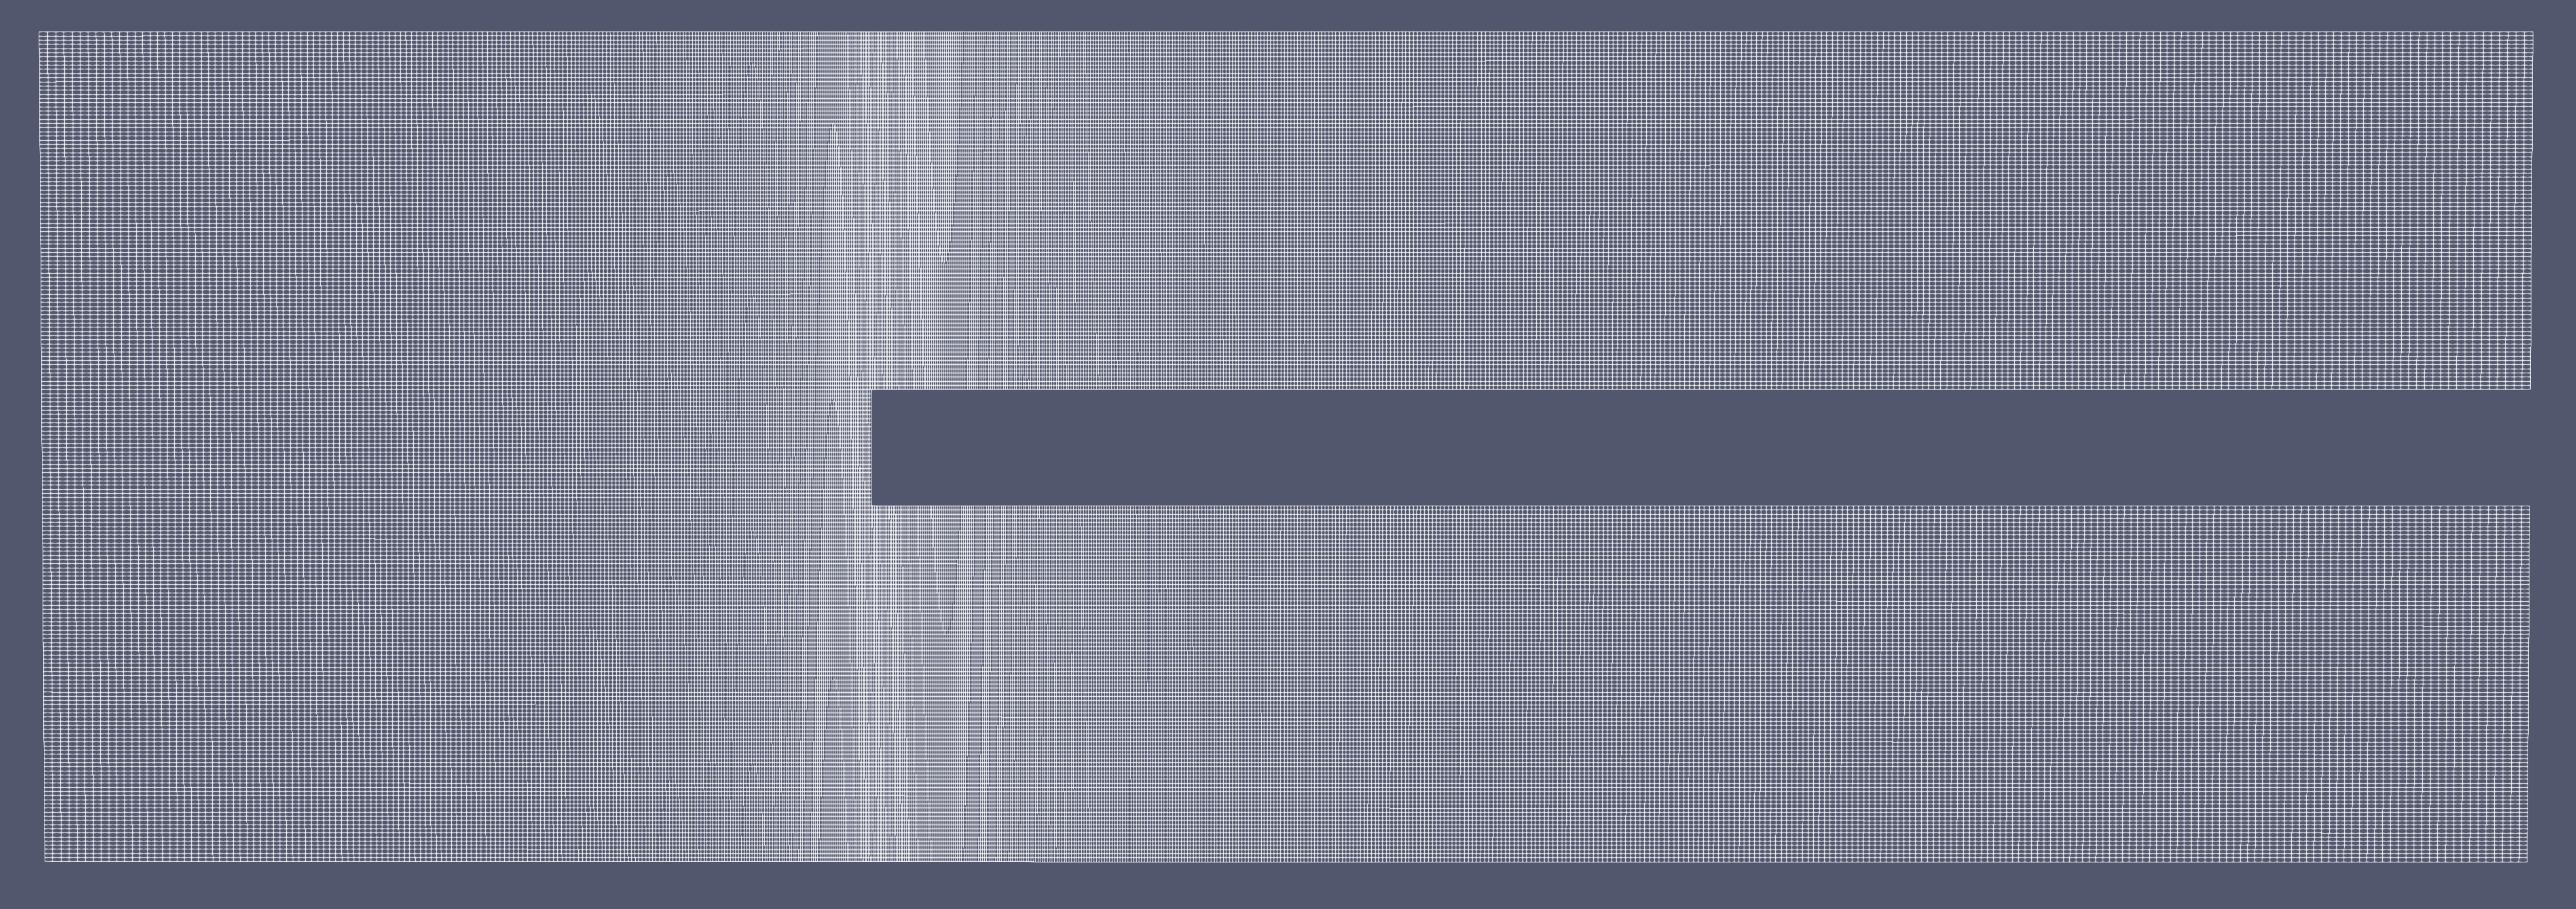
\includegraphics[width=1\linewidth]{pv-mesh.png}
	\caption{Síť řešeného modelu}
	\label{fig:pvmesh}
\end{figure}


Okrajové podmínky pro jednotlivé veličiny, pro nás primárně pro rychlost $U$ a tlak $p$  jsou definovány v souborech ve složce \texttt{0}.

Ostatní parametry řešiče úlohy, netýkající se přímo lineárních řešičů jsou pro všechny simulace totožné a jsou v souborech \texttt{transportProperties}, \texttt{turbulenceProperties}, \texttt{fvSchemes} a \texttt{controlDict}. Zde uvedeme jen vybrané parametry popisující naší úlohu.

\begin{itemize}
	\item{\makebox[5cm]{application:\hfill}simpleFoam}
	\item{\makebox[5cm]{simulationType:\hfill}RAS}
	\item{\makebox[5cm]{RASmodel:\hfill}kEpsilon}
	\item{\makebox[5cm]{turbulence:\hfill}on}
	\item{\makebox[5cm]{transportModel:\hfill}Newtonian}
	\item{\makebox[5cm]{nu:\hfill}1e-05}
\end{itemize}


	
Na ukázku je zde obrázek \ref{fig:pv-GAMG-GS} výsledného klidového stavu pořízený v ParaView. Výsledky úlohy řešené pomocí různých lineárních řešičů vypadají prakticky identicky.
	
	 \begin{figure}[H]
		\centering
		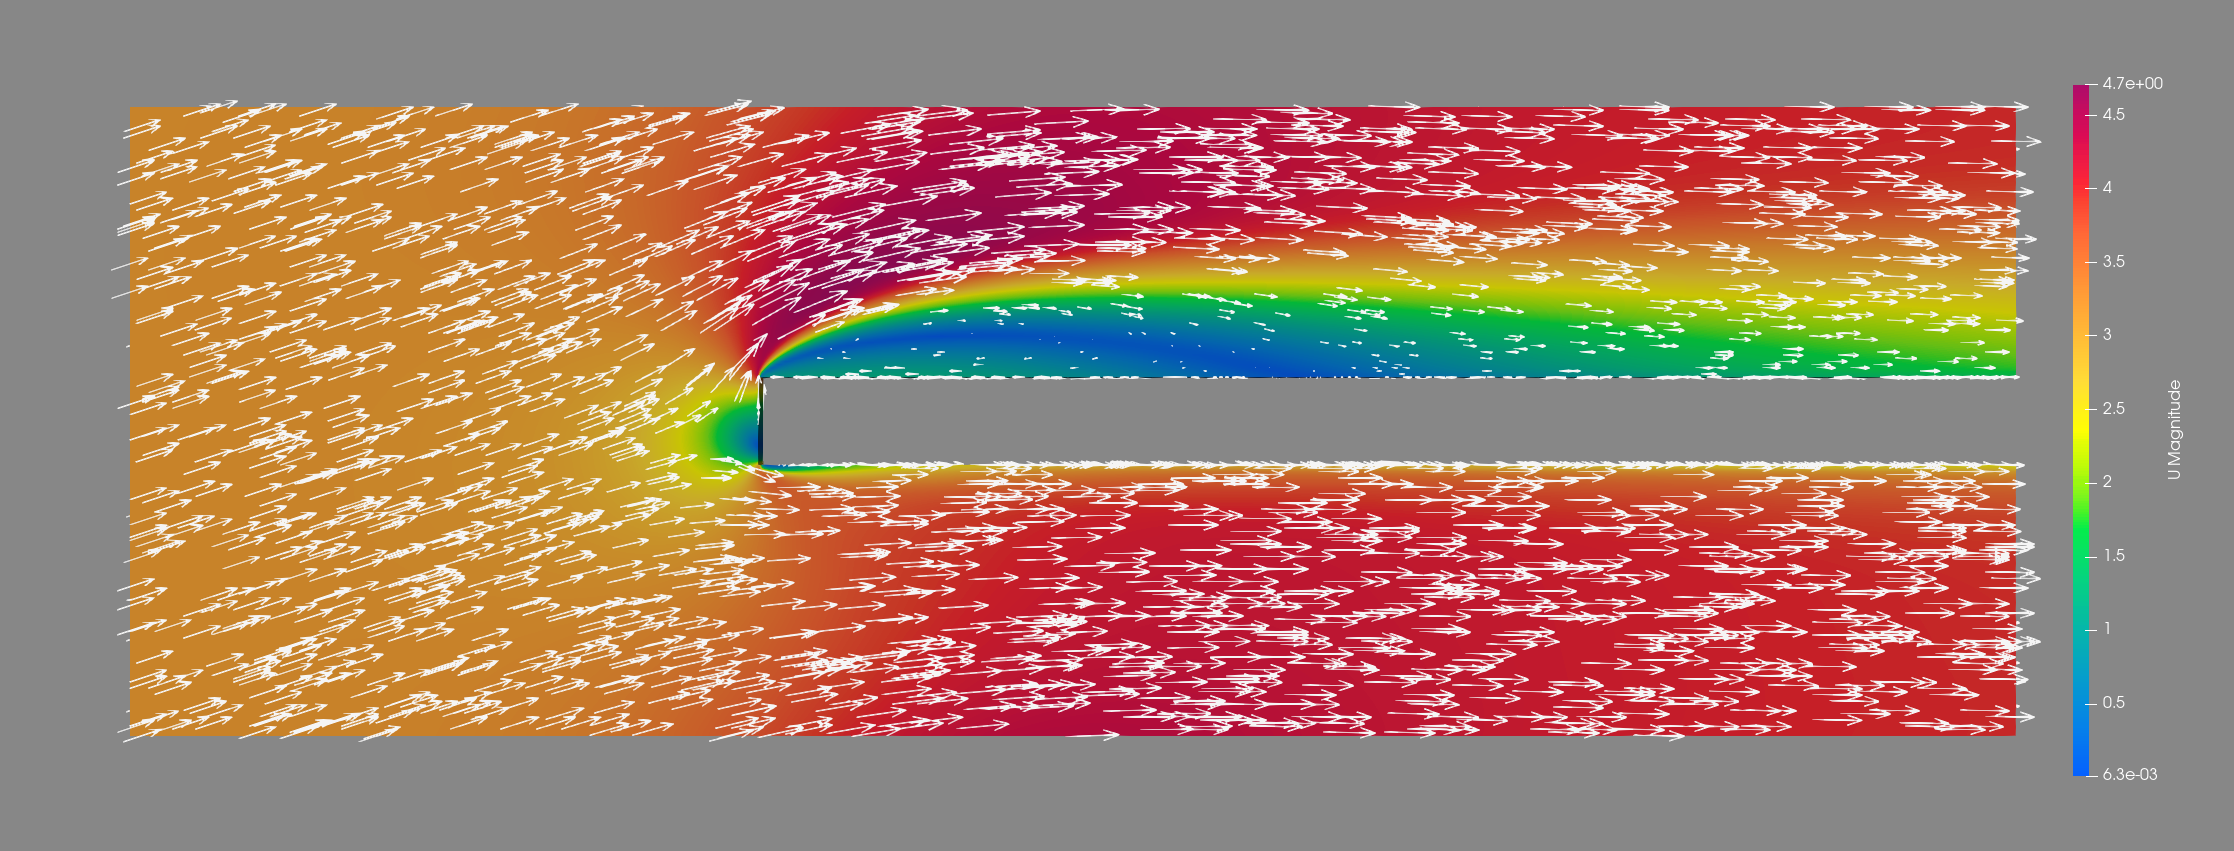
\includegraphics[width=1\linewidth]{pv-GAMG-GS.png}
		\caption{Klidový stav s vektory rychlosti $U$ v ParaView}
		\label{fig:pv-GAMG-GS}
	\end{figure}


Na lineárních řešičích budeme zkoumat vliv následujících parametrů na konvergenci simulace:
 
\begin{itemize}
	\item typ použitého řešiče
	\item typ použitého předpodmiňovače
	\item typ použitého smootheru
	\item hodnotu pod-relaxace
\end{itemize}

Nastavení řešičů se v OpenFOAM dělá v souboru \texttt{system/fvSolution}. Ukázkový soubor je v příloze \ref{app:fvsol}.
	
 Nejprve nás zajímá typ použitého řešiče, případně přidruženého předpodmiňovače nebo smootheru. V tabulkách \ref{table:solvers_GAMG}, \ref{table:solvers_PCG} a \ref{table:solvers_smooth} jsou uvedená nastavení a výsledné počty iterací řešení úlohy a čas běhu simulace testovací úlohy.
 
 Konvergenci metody měříme pomocí počtu využitých iterací metody. Maximální počet iterací byl nastaven na $500$. Tolerance lineárního řešiče je shodně nastavena na $10^{-6}$, relativní tolerance na $0$. Velikost reziduí v rámci SIMPLE algoritmu pomocí \texttt{residualControl} parametru pro tlak $p$ nastaveno na $10^{-3}$ a pro rychlost $U$ na $10^{-4}$.

 \begin{table}[H]
	\centering
	\caption{Nastavení lineárních řešičů pro jednotlivé simulace}
	\renewcommand{\arraystretch}{1.9}
	\begin{tabular}{*7c}
		\toprule
		%\multicolumn{2}{c}{\textbf{Řešič pro $p$}} & \multicolumn{2}{c}{\textbf{Řešič pro $U$}}\\
		\multicolumn{2}{c}{Tlak $p$: \textbf{GAMG}} & \multicolumn{2}{c}{Rychlost $U$: \textbf{GAMG}}\\		
		\midrule
		%\textit{Předpod.}&\textit{Smoother}&\textit{Předpod.}&\textit{Smoother}&\textit{Relaxace}&\textit{ \# iter}&\textit{čas}\\
		Předpod.&Smoother&Předpod.&Smoother&\# iter&Čas\\
		\midrule
 --- & DIC & --- &  DILU & 475 &157.94\\		
 --- & GaussSeidel &  --- & GaussSeidel & 475&176.99\\
		
			\bottomrule
\end{tabular}

\label{table:solvers_GAMG}

\end{table}


\begin{table}[H]
\centering
\caption{Nastavení lineárních řešičů pro jednotlivé simulace}
\renewcommand{\arraystretch}{1.9}
\begin{tabular}{*7c}
\toprule	

%\multicolumn{2}{c}{\textbf{}} & \multicolumn{2}{c}{\textbf{Řešič pro $U$}}\\
\multicolumn{2}{c}{Tlak $p$: \textbf{PCG}} & \multicolumn{2}{c}{Rychlost $U$: \textbf{PBiCG}}\\		
\midrule
%\textit{Předpod.}&\textit{Smoother}&\textit{Předpod.}&\textit{Smoother}&\textit{Relaxace}&\textit{ \# iter}&\textit{čas}\\
Předpod.&Smoother&Předpod.&Smoother&\# iter&Čas\\
\midrule
 DIC & --- &  DILU & --- &474&540.48\\								
FDIC & --- &  DILU & --- &474&531.14\\	
 \shortstack{GAMG\\GS smooth.}& --- &  \shortstack{GAMG\\GS smooth.}& --- &475&184.85\\	
diagonal & --- & diagonal & ---&474&679.26\\	

		\bottomrule
\end{tabular}

\label{table:solvers_PCG}

\end{table}

Z výsledků je patrné, že pro naši úlohu ideální GAMG řešič, což odpovídá i obecným doporučením pro řešení úloh pro klidový stav. PCG/PBiCG řešiče dospějí ke stejným výsledkům, v podobném počtu iterací, jen za víc jak dvojnásobný čas. Obecně al GAMG není tak dobře škálovatelný jaklo PCG/PBiCG a je tedy proto možné, že pro jinou úlohu, případě i stejnou úlohu ale řádově větší síť by mohl být PCG/PBiCG řešič vhodnější.

Na obrázku \ref{fig:p-residuum} jsou zobrazeny průběhy simulací pomocí závislosti velikosti rezidua pro tlak $p$ a různé řešiče. Na obrázku \ref{fig:ux-residuum} je pak totéž, jen pro rychlost v $x$ové souřadnici $U_x$.


\begin{figure}[H]
	\centering
	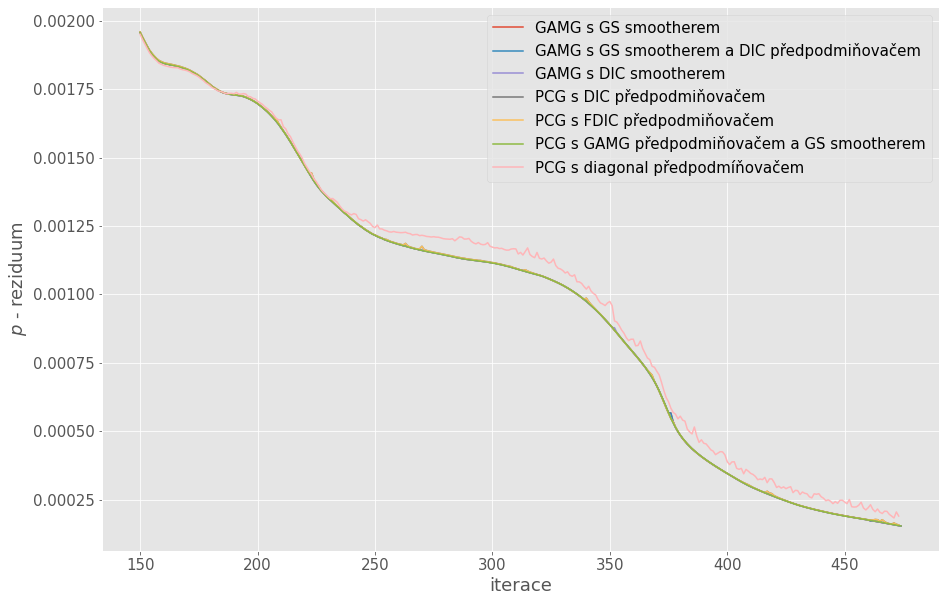
\includegraphics[width=1\linewidth]{p-residuum.png}
	\caption{Konvergence lineárních řešičů v různé konfiguraci pro tlak $p$}
	\label{fig:p-residuum}
\end{figure}


\begin{figure}[H]
	\centering
	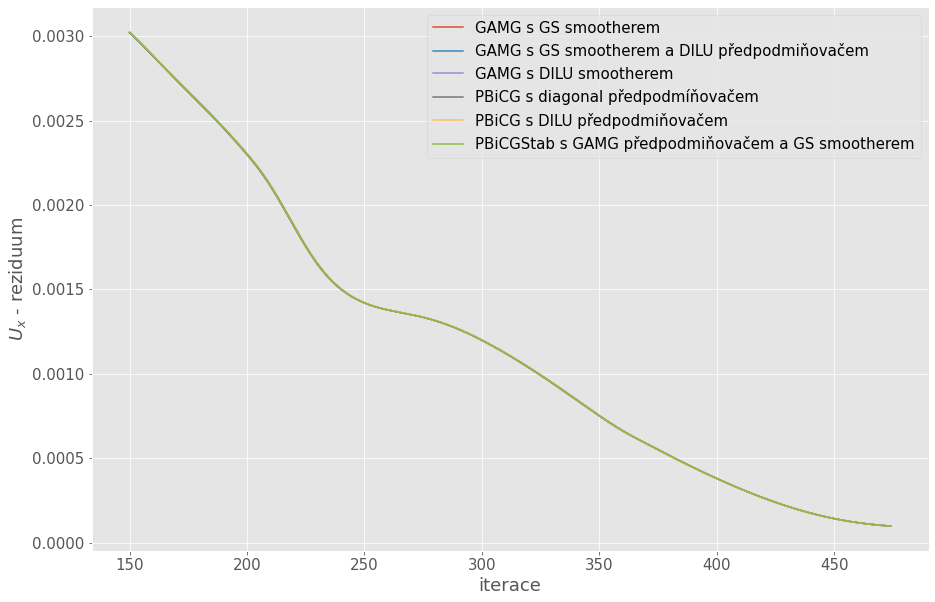
\includegraphics[width=1\linewidth]{ux-residuum.png}
	\caption{Konvergence lineárních řešičů v různé konfiguraci pro rychlost $U_x$}
	\label{fig:ux-residuum}
\end{figure}

Z výsledků v tabulce \ref{table:solvers_smooth} je vidět, že smoothSolver není pro naši úlohu vhodný. Ani v jednom případě nedokonvergovala úloha ke stacionárnímu stavu v stanovém maximálním počtu 500 iterací.  I čas potřebný ke zpracování této úlohy je výrazně vyšší. 

 \begin{table}[H]
	\centering
	\caption{Nastavení lineárních řešičů pro jednotlivé simulace}
	\renewcommand{\arraystretch}{1.9}
	\begin{tabular}{*7c}
		\toprule
\multicolumn{2}{c}{Tlak $p$: \textbf{smoothSolver}} & \multicolumn{2}{c}{Rychlost $U$: \textbf{smoothSolver}}\\
%\multicolumn{2}{c}{\textbf{Řešič pro $p$}} & \multicolumn{2}{c}{\textbf{Řešič pro $U$}}\\
%\multicolumn{2}{c}{\textbf{smoothSolver}} & \multicolumn{2}{c}{\textbf{smoothSolver}}\\		
\midrule
%\textit{Předpod.}&\textit{Smoother}&\textit{Předpod.}&\textit{Smoother}&\textit{Relaxace}&\textit{ \# iter}&\textit{čas}\\
Předpod.&Smoother&Předpod.&Smoother&\# iter&Čas\\
\midrule		
 --- & DIC &  --- & GaussSeidel &500+&1136.21\\	
 --- & DIC & --- & DILU &500+&1039.73\\
 --- & GaussSeidel &   --- & GaussSeidel &500+&1011.42\\		
 FDIC & GaussSeidel &  --- & GaussSeidel &500+&1008.47\\
 --- & \shortstack{symGauss-\\Seidel} &  --- & \shortstack{symGauss-\\Seidel}&500+&1370.58\\	
\bottomrule
\end{tabular}
	
	\label{table:solvers_smooth}
\end{table}

Na obrázcích \ref{fig:p-residuum-smooth} (pro tlak $p$) a \ref{fig:ux-residuum-smooth} (pro rychlost $U_x$) je vidět proč smooth řešič nekonverguje, nebo konverguje velmi pomalu. V obou sledovaných veličinách reziduum osciluje a jeho hodnota se snižuje velmi pomalu.

\begin{figure}[H]
	\centering
	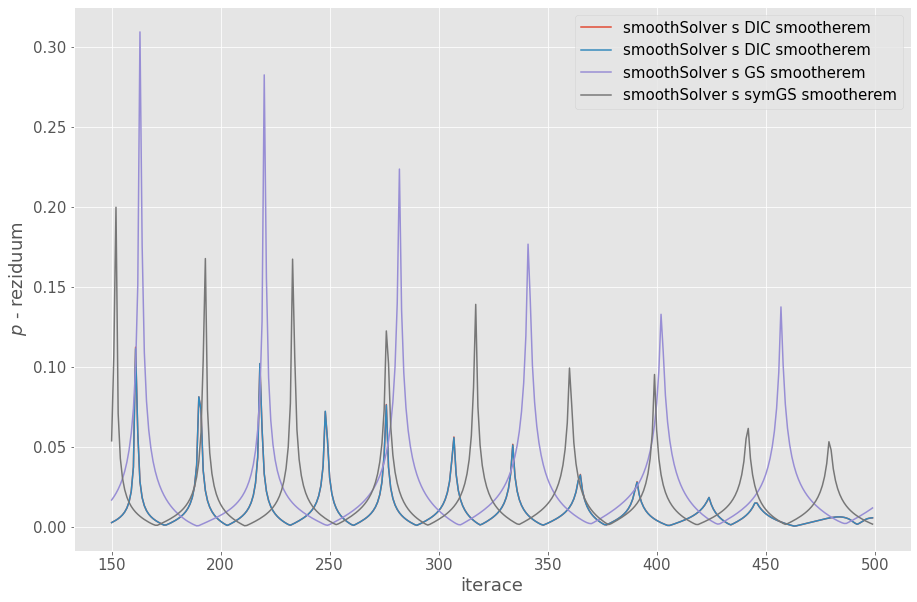
\includegraphics[width=1\linewidth]{p-residuum-smooth.png}
	\caption{Konvergence lineárních řešičů smoothSolver v různé konfiguraci pro tlak $p$}
	\label{fig:p-residuum-smooth}
\end{figure}

\begin{figure}[H]
	\centering
	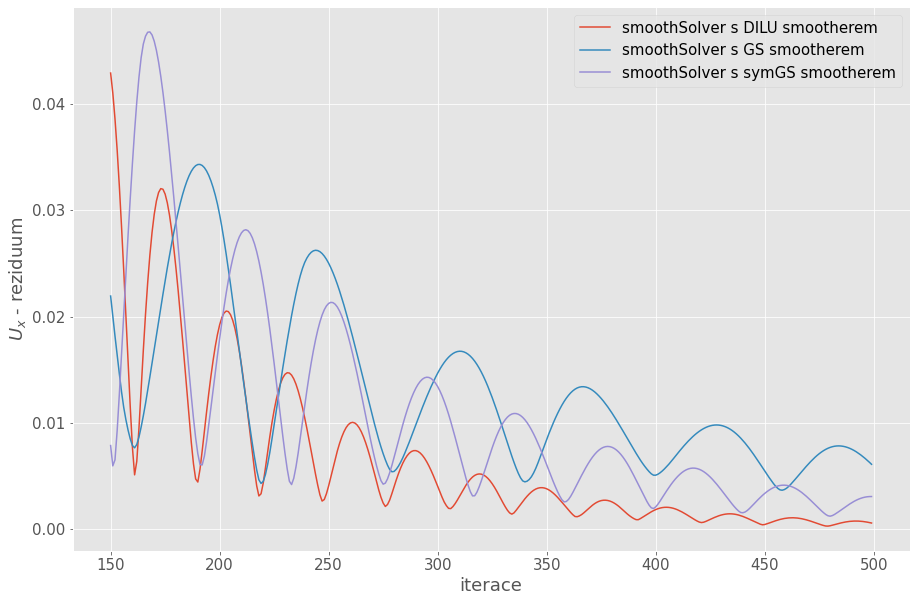
\includegraphics[width=1\linewidth]{ux-residuum-smooth.png}
	\caption{Konvergence lineárních řešičů smoothSolver v různé konfiguraci pro rychlost $U_x$}
	\label{fig:ux-residuum-smooth}
\end{figure}
	


Na GAMG řešiči si ukážeme vliv hodnoty relaxace. Obecně platí, že vyšší relaxace zvyšuje rychlost konvergence, nižší metodu zestabilní. V tabulce \ref{table:solvers_gamg_relax} jsou výsledky pro různé hodnoty relaxačního parametru v porovnání s defaultní hodnotou $0.9$. 

 \begin{table}[H]
	\centering
	\caption{Nastavení lineárních řešičů pro jednotlivé simulace}
	\renewcommand{\arraystretch}{1.9}
	\begin{tabular}{*8c}
		\toprule
		\multicolumn{2}{c}{Tlak $p$: \textbf{GAMG}} & \multicolumn{2}{c}{Rychlost $U$: \textbf{GAMG}}\\		
		\midrule
		%\textit{Předpod.}&\textit{Smoother}&\textit{Předpod.}&\textit{Smoother}&\textit{Relaxace}&\textit{ \# iter}&\textit{čas}\\
		Předpod.&Smoother&Předpod.&Smoother&Relaxace& \# iter&Čas\\
		
		\midrule
		
		--- & GaussSeidel &  --- & GaussSeidel & 0.9&475&176.99\\
		--- & GaussSeidel &  --- & GaussSeidel & 0.3&500+&151.49\\
		--- & GaussSeidel &  --- & GaussSeidel & 0.95&285&114.15\\
		--- & GaussSeidel &  --- & GaussSeidel & 0.98&500+&257.28\\		
		%%%%DIC & GaussSeidel &  DILU & GaussSeidel & 0.98&475&160.59\\
		\bottomrule
	\end{tabular}
	
	\label{table:solvers_gamg_relax}
	
\end{table}

Ideální hodnotou pro nejrychlejší konvergenci je $0.95$, úloha dokoverguje v 285 iteracích za přibližně $114s$. Hodnota relaxace $0.3$ je moc nízká na to, aby úloha dokonvergovala v maximálním počtu 500 iterací.  Hodnota $0.98$ je naopak moc vysoká a reziduum úlohy se rozkmitá a řešení nekonverguje, jak je vidět z obrázků \ref{fig:p-residuum-relax} a \ref{fig:ux-residuum-relax}.

\begin{figure}[H]
	\centering
	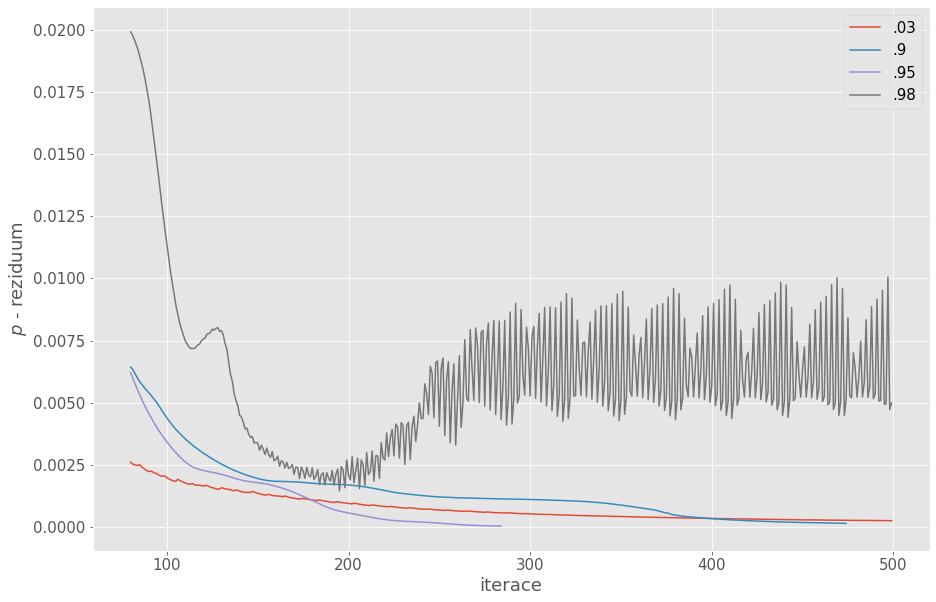
\includegraphics[width=1\linewidth]{p-under-relax.png}
	\caption{Konvergence lineárních řešičů smoothSolver v různé konfiguraci pro rychlost $U_x$}
	\label{fig:p-residuum-relax}
\end{figure}

\begin{figure}[H]
	\centering
	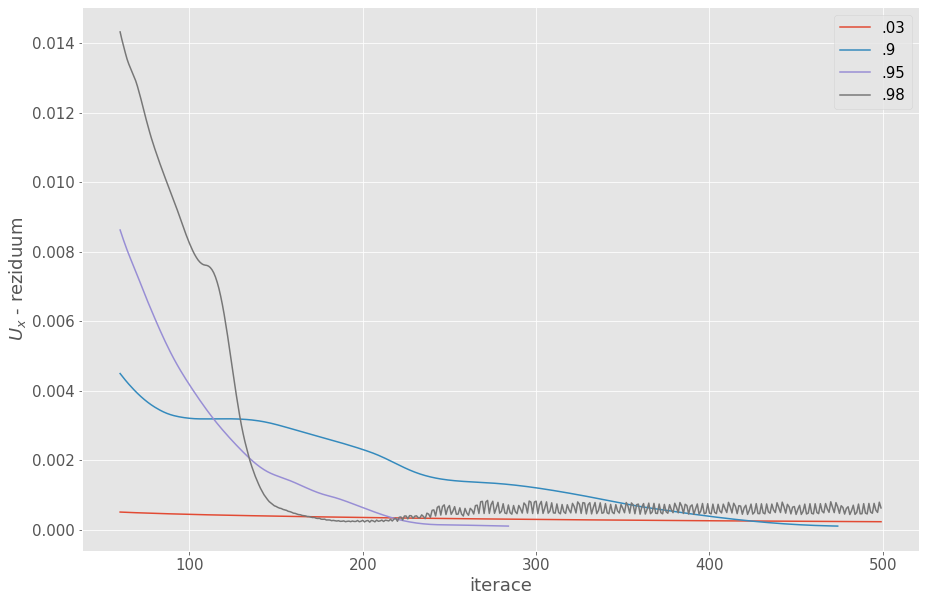
\includegraphics[width=1\linewidth]{ux-under-relax.png}
	\caption{Konvergence lineárních řešičů smoothSolver v různé konfiguraci pro rychlost $U_x$}
	\label{fig:ux-residuum-relax}
\end{figure}

Zdálo by se, že použít relaxaci na \uv{opravení} smooth řešiče je dobrý nápad. Z tabulky \ref{table:solvers_set3}  je ale vidět, že se výsledky nijak nezlepší.

\begin{table}[H]
	\centering
	\caption{Nastavení lineárních řešičů pro jednotlivé simulace}
	\renewcommand{\arraystretch}{1.9}
	\begin{tabular}{*8c}
		\toprule
		\multicolumn{2}{c}{Tlak $p$: \textbf{smoothSolver}} & \multicolumn{2}{c}{Rychlost $U$: \textbf{smoothSolver}}\\
		\midrule
		%\textit{Předpod.}&\textit{Smoother}&\textit{Předpod.}&\textit{Smoother}&\textit{Relaxace}&\textit{ \# iter}&\textit{čas}\\
		Předpod.&Smoother&Předpod.&Smoother&Relaxace& \# iter&Čas\\
		\midrule
		--- & GaussSeidel &   --- & GaussSeidel &0.9&500+&1011.42\\
		--- & GaussSeidel &  --- & GaussSeidel &0.3&500+&951.71\\
		--- & GaussSeidel &   --- & GaussSeidel &0.95&500+&1086.7\\
		--- & GaussSeidel &  --- & GaussSeidel &0.98&500+&1222.24\\
		FDIC & GaussSeidel &  --- & GaussSeidel &0.9&500+&1008.47\\
		\bottomrule
	\end{tabular}
	
	\label{table:solvers_set3}
\end{table}

Další parametr, který popíše \uv{úspěšnost} lineárního řešiče při řešení úlohy je počet iteračních kroků lineárního řešiče v rámci časových kroků metody. V každém kroku řeší lineární řešič soustavu a zastaví iterování v chvíli, kdy dosáhne nastavené tolerance. Na obrázcích \ref{fig:p-iters-1} a \ref{fig:p-iters-2} je vidět tato závislost pro řešení tlaku $p$, na obrázku \ref{fig:ux-iters} pak pro rychlost $U_x$. Ze všech tří grafů opět vyplývá, že GAMG řešič dosahuje nejlepší konvergence. Naopak smoothSolver naráží ve všech časových iterací metody na maximální možnou hodnotu iterací řešiče $1000$.

\begin{figure}[H]
	\centering
	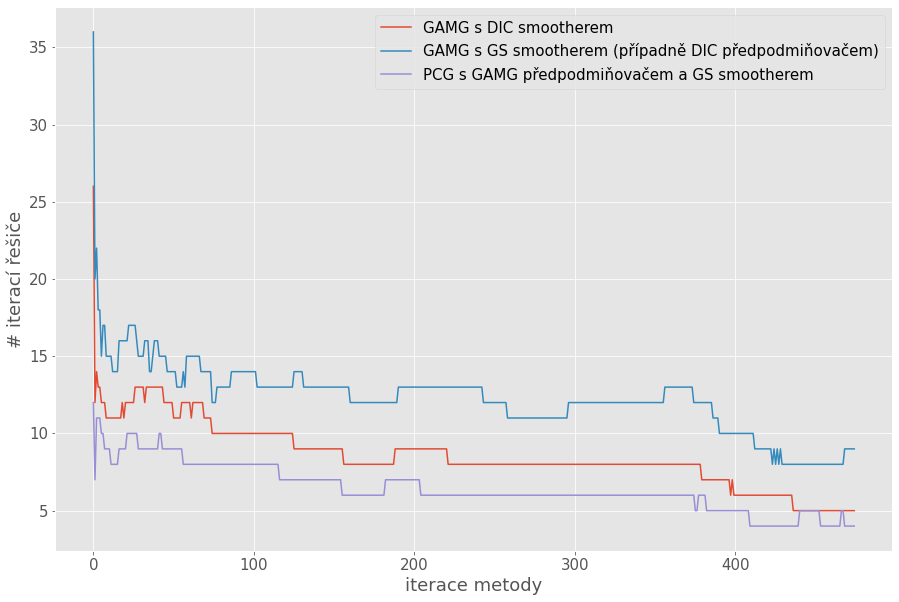
\includegraphics[width=1\linewidth]{p-solver-iters-1.png}
	\caption{Počet iterací lineárního řešiče v závislosti na iteraci metody pro tlak $p$}
	\label{fig:p-iters-1}
\end{figure}

\begin{figure}[H]
	\centering
	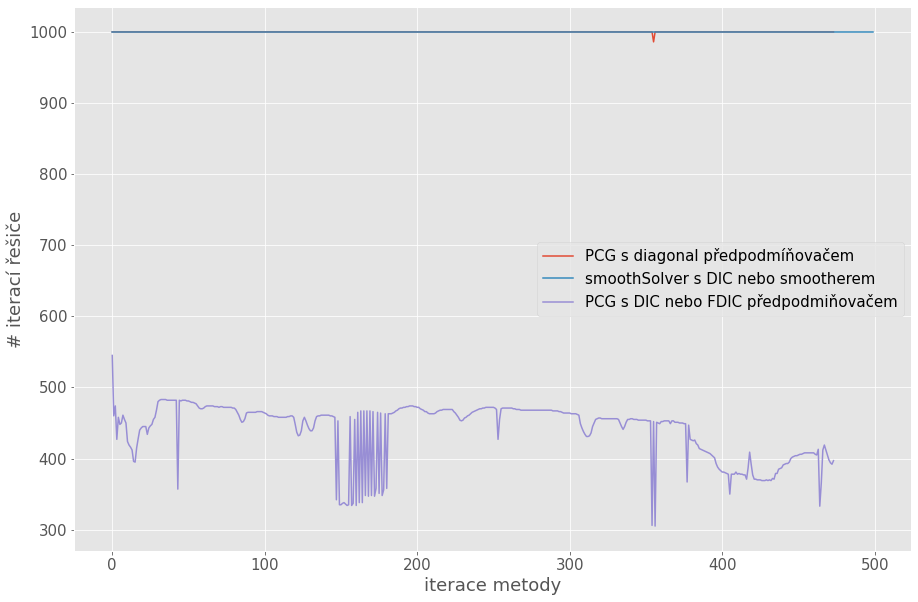
\includegraphics[width=1\linewidth]{p-solver-iters-2.png}
	\caption{Počet iterací lineárního řešiče v závislosti na iteraci metody pro tlak $p$}
	\label{fig:p-iters-2}
\end{figure}

\begin{figure}[H]
	\centering
	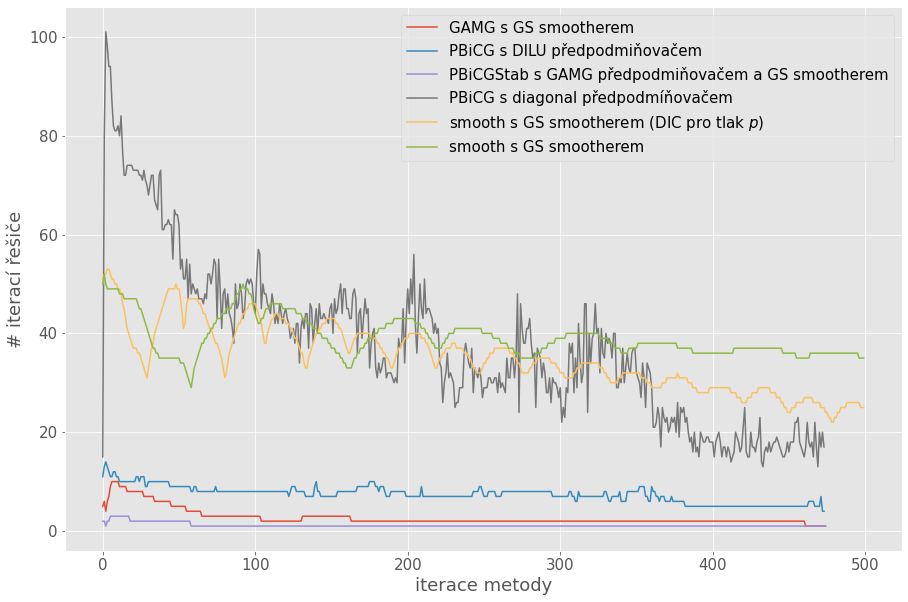
\includegraphics[width=1\linewidth]{ux-solver-iters.png}
	\caption{Počet iterací lineárního řešiče v závislosti na iteraci metody pro rychlost $U_x$}
	\label{fig:ux-iters}
\end{figure}



{\let\clearpage\relax \chapter{Závěr}}

Ukázali jsme, jakými parametry lineárních řešičů se dá ovlivnit výsledná konvergence úlohy. Obecně nelze říci, který řešič je nejvhodnější a to ani pro konkrétní úlohu. Pro naši ukázkovou úlohu proudění v lopatkové mříži a pro konkrétní síť je nejvhodnější GAMG řešič s GaussSeidel smootherem a relaxací nastavenou na $0.95$. Tato volba ale nemusí být optimální pro jinou síť, jinak nastavené parametry turbulence nebo i jiný hardware, na kterém úlohu řešíme. Předchozí text by tedy měl sloužit přinejlepším jen jako přehled a ukázka řešičů dostupných v OpenFOAM.



\newpage
\appendix

{\let\clearpage\relax \chapter{blockMeshDict}\label{app:blockmeshdict}}
\begin{verbatim}
/*---------------------------*- C++ -*-----------------------------*\
| =========                 |                                                 |
| \\      /  F ield         | OpenFOAM: The Open Source CFD Toolbox           |
|  \\    /   O peration     | Version:  v2006                                 |
|   \\  /    A nd           | Website:  www.openfoam.com                      |
|    \\/     M anipulation  |                                                 |
\*-----------------------------------------------------------------*/
FoamFile
{
	version         2.0;
	format          ascii;
	class           dictionary;
	object          blockMeshDict;
}
// * * * * * * * * * * * * * * * * * * * * * * * * * * * * * * * * //

scale   1;

vertices
(
(0 0    0)
(1 0    0)
(3 0    0)
(3 0.43 0)
(1 0.43 0)
(1 0.57 0)
(3 0.57 0)
(3 1    0)
(1 1    0)
(0 1    0)
(0 0.57 0)
(0 0.43 0)


(0 0    0.1)
(1 0    0.1)
(3 0    0.1)
(3 0.43 0.1)
(1 0.43 0.1)
(1 0.57 0.1)
(3 0.57 0.1)
(3 1    0.1)
(1 1    0.1)
(0 1    0.1)
(0 0.57 0.1)
(0 0.43 0.1)


);

blocks
(
hex (0 1 4 11 12 13 16 23) (200 86 1) simpleGrading (0.2 1 1)
hex (1 2 3 4 13 14 15 16) (400 86 1) simpleGrading (5 1 1)
hex (11 4 5 10 23 16 17 22) (200 28 1) simpleGrading (0.2 1 1)
hex (10 5 8 9 22 17 20 21) (200 86 1) simpleGrading (0.2 1 1)
hex (5 6 7 8 17 18 19 20) (400 86 1) simpleGrading (5 1 1)
);

edges
(
);

boundary
(
frontAndBack
{
	type empty;
	faces
	(
	(0 1 4 11)
	(1 2 3 4)
	(11 4 5 10)
	(10 5 8 9)
	(5 6 7 8)
	
	(12 13 16 23)
	(13 14 15 16)
	(23 16 17 22)
	(22 17 20 21)
	(17 18 19 20)
	);
}

top	
{
	type cyclic;
	neighbourPatch bottom;
	faces
	(
	(9 8 20 21)
	(8 7 19 20)
	);
}

bottom	
{
	type cyclic;
	neighbourPatch top;
	faces
	(
	(0 1 13 12)
	(1 2 14 13)
	);
}

fixedBalk
{
	type wall;
	faces
	(
	(5 6 18 17)
	(4 5 17 16)
	(4 3 15 16)
	);	
}

outlet
{
	type patch;
	faces
	(
	(6 7 19 18)
	(2 3 15 14)
	);
}

inlet
{
	type patch;
	faces
	(
	(0 11 23 12)
	(11 10 22 23)
	(10 9 21 22)
	);
}
);
mergePatchPairs
(
);

// ************************************************************** //
\end{verbatim}

{\let\clearpage\relax \chapter{fvSolution}\label{app:fvsol}}
\begin{verbatim}
	/*---------------------------*- C++ -*-----------------------------*\
	| =========                 |                                                 |
	| \\      /  F ield         | OpenFOAM: The Open Source CFD Toolbox           |
	|  \\    /   O peration     | Version:  v2006                                 |
	|   \\  /    A nd           | Website:  www.openfoam.com                      |
	|    \\/     M anipulation  |                                                 |
	\*-----------------------------------------------------------------*/
	FoamFile
	{
		version     2.0;
		format      ascii;
		class       dictionary;
		location    "system";
		object      fvSolution;
	}
	// * * * * * * * * * * * * * * * * * * * * * * * * * * * * * * * * //
	
	solvers
	{
		p
		{
			solver          smoothSolver;
			smoother        GaussSeidel;
			tolerance       1e-06;
			relTol          0; 
		}
		
		"(U|k|epsilon|omega|f|v2)"
		{
			solver          smoothSolver;
			smoother        GaussSeidel;
			tolerance       1e-06;
			relTol          0; 
		}
	}
	
	SIMPLE
	{
		nNonOrthogonalCorrectors 0;
		consistent      yes;
		
		residualControl
		{
			p               1e-3;
			U               1e-4;
			"(k|epsilon|omega|f|v2)" 1e-4;
		}
	}
	
	relaxationFactors
	{
		equations
		{
			U               .95; 
			".*"            .95;
		}
	}
	
	
	// ************************************************************** //
\end{verbatim}
	
\end{document}